\section{\texorpdfstring{$L^1$}{L1}中的Fourier变换}
\label{sec:fourier-l1}

非周期函数不能在一个周期上读坐标，但上一节末尾已经提示了办法：周期$T$越长，频率$k/T$越密。对定义在整个$\mathbb R^d$上的函数，频率应当取遍$\mathbb R^d$，对整数$k$的求和换成对频率$\xi$的积分。向量的下标从整数连成了整个空间，这是类比的又一次推广，也是它开始变得不严格的地方。

本节先在绝对可积函数上建立变换本身，再单独回答怎样从频率函数还原原函数。

\subsection{Fourier变换的基本性质}
\label{sec:fourier-l1-properties}

\paragraph{定义与归一化}

先用一个周期很长的函数看看下标是怎样连起来的。设$f$是实轴上的可积函数，支撑在$[-T/2,T/2]$内，把它按$T$周期延拓。由式~\eqref{eq:fourier-period-T}，它的系数$c_k$乘$T$之后是
\[
Tc_k=\int_{-T/2}^{T/2}f(x)\,e^{-2\pi\mathrm i(k/T)x}\,\mathrm dx .
\]
只要$T$足够大，右边的积分就不再依赖$T$，它只依赖频率$\xi=k/T$，是同一个函数$\xi\mapsto\int f(x)e^{-2\pi\mathrm ix\xi}\,\mathrm dx$在格点$k/T$上的取值。

取方框$B=\mathbf 1_{[-1/2,1/2]}$算一个具体的值。取$T=2$、$k=1$，频率是$\xi=1/2$，于是
\[
2c_1=\int_{-1/2}^{1/2}e^{-\mathrm i\pi x}\,\mathrm dx=\frac{\sin(\pi/2)}{\pi/2}=\frac2\pi\approx0.637.
\]
图~\ref{fig:fourier-series-to-transform}画出$T=2,4,8$时的全部$Tc_k$：它们落在同一条曲线上，$T$每增大一倍，取样点就密一倍。

\begin{BookInlineFigure}
  \centering
  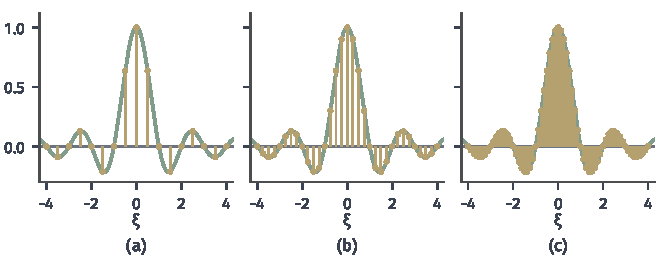
\includegraphics[width=112mm]{figures/04-spaces-measures-and-geometry/03-function-spaces/matplotlib/fourier-series-to-transform/figure.pdf}
  \caption{周期增大时系数连成曲线。方框$B$按周期$T$延拓，黄色竖线为$Tc_k$，位于频率$k/T$处。(a)$T=2$。(b)$T=4$。(c)$T=8$。绿色曲线是极限对象$\sin(\pi\xi)/(\pi\xi)$，三幅图中相同。}
  \label{fig:fourier-series-to-transform}
\end{BookInlineFigure}

展开式也随之变形。把$c_k$代入周期$T$的Fourier级数，得到
\[
f(x)=\sum_{k\in\mathbb Z}\Bigl(\int f(y)e^{-2\pi\mathrm i(k/T)y}\,\mathrm dy\Bigr)\,e^{2\pi\mathrm i(k/T)x}\cdot\frac1T .
\]
右边是一个频率步长为$1/T$的Riemann和。$T\to\infty$时，它的形式极限是对$\xi$的积分。这只是启发，下面的定义和证明不依赖这个极限过程。

对$x,\xi\in\mathbb R^d$，记$x\cdot\xi=\sum_ix_i\xi_i$。函数$x\mapsto e^{2\pi\mathrm ix\cdot\xi}$沿方向$\xi/\lvert\xi\rvert$每前进$1/\lvert\xi\rvert$就转一圈，所以$\lvert\xi\rvert$是单位长度内的圈数，这样的函数称为平面波。

\begin{definition}[Fourier变换]
\label{def:fourier-transform-l1}
对$f\in L^1(\mathbb R^d)$，定义它的\term{Fourier变换}（Fourier transform）为
\begin{equation}
\widehat f(\xi)=\int_{\mathbb R^d}f(x)e^{-2\pi\mathrm ix\cdot\xi}\,\mathrm dx ,\qquad\xi\in\mathbb R^d .
\label{eq:fourier-transform-l1}
\end{equation}
\end{definition}

由于指数因子的模恒为$1$，可积性保证积分对每个$\xi$都存在，并且改变$f$在零测集上的值不影响结果。所以$\widehat f$是一个在每个频率处都有确定值的函数，这一点到$L^2$情形会改变。

类比在这里要打一个折扣。式~\eqref{eq:fourier-transform-l1}形式上是“与平面波作内积”，但平面波的模恒为$1$，在$\mathbb R^d$上既不可积也不平方可积，它们不是$L^2(\mathbb R^d)$中的元素，更谈不上构成正交基。可以把$\widehat f(\xi)$想成下标为$\xi$的坐标，但一切结论都要直接证明，不能照搬Hilbert空间的展开定理。

指数中的$2\pi$是一种约定。另一种常见写法用角频率$\omega=2\pi\xi$，把指数换成$e^{-\mathrm ix\cdot\omega}$，所得函数记为$F(\omega)$，两者只差自变量的伸缩，$F(\omega)=\widehat f(\omega/2\pi)$。约定不改变任何结论，只改变反演与能量公式中的常数；本章始终采用定义中的写法，第~\ref{sec:fourier-l2}节末尾给出常数的对照。

\paragraph{有界性、连续性与高频衰减}

和周期情形一样，可积性已经足以给出变换的几条基本性质。

\begin{theorem}[$L^1$上Fourier变换的基本性质]
\label{thm:fourier-l1-properties}
设$f,g\in L^1(\mathbb R^d)$，$a,b\in\mathbb C$。则
\begin{enumerate}
\item $\widehat{af+bg}=a\widehat f+b\widehat g$，且$\lVert\widehat f\rVert_\infty\leq\lVert f\rVert_1$；
\item $\widehat f$在$\mathbb R^d$上连续；
\item $\lvert\xi\rvert\to\infty$时$\widehat f(\xi)\to0$。
\end{enumerate}
\end{theorem}

\begin{proof}
线性来自积分的线性。有界性来自
\[
\lvert\widehat f(\xi)\rvert\leq\int_{\mathbb R^d}\lvert f(x)e^{-2\pi\mathrm ix\cdot\xi}\rvert\,\mathrm dx=\lVert f\rVert_1.
\]

连续性：若$\xi_n\to\xi$，被积函数逐点收敛到$f(x)e^{-2\pi\mathrm ix\cdot\xi}$，并被可积函数$\lvert f\rvert$控制。由控制收敛定理，$\widehat f(\xi_n)\to\widehat f(\xi)$。

高频衰减与引理~\ref{lem:fourier-riemann-lebesgue}的证明相同。对$\xi\neq0$取
\[
h=\frac{\xi}{2\lvert\xi\rvert^2},
\]
则$e^{-2\pi\mathrm ih\cdot\xi}=e^{-\pi\mathrm i}=-1$。作换元$x\mapsto x+h$，得到
\[
\widehat f(\xi)=-\int_{\mathbb R^d}f(x+h)\,e^{-2\pi\mathrm ix\cdot\xi}\,\mathrm dx.
\]
与原式相加再取模，得到
\[
2\lvert\widehat f(\xi)\rvert\leq\int_{\mathbb R^d}\lvert f(x)-f(x+h)\rvert\,\mathrm dx.
\]
$\lvert\xi\rvert\to\infty$时$\lvert h\rvert=1/(2\lvert\xi\rvert)\to0$，由第~\ref{chap:smoothing-weak-derivatives}章的平移积分连续性，右边趋于零。
\end{proof}

于是$f\mapsto\widehat f$把$L^1(\mathbb R^d)$线性地映到在无穷远处趋于零的有界连续函数中，而且不增加相应的范数。第3条也称为Riemann--Lebesgue引理。它不给出衰减速度，速度与$f$的光滑性有关，第~\ref{sec:fourier-operations}节的微分规则会给出具体联系。

\paragraph{三个例子}

先算两个一维例子。第一个是中心方框$B=\mathbf 1_{[-1/2,1/2]}$。直接积分，对$\xi\neq0$有
\begin{equation}
\widehat B(\xi)=\int_{-1/2}^{1/2}e^{-2\pi\mathrm ix\xi}\,\mathrm dx=\frac{\sin(\pi\xi)}{\pi\xi},
\label{eq:fourier-box}
\end{equation}
并且$\widehat B(0)=1$。零点在非零整数处，例如$\widehat B(1/2)=2/\pi$，与上面周期化时算出的$2c_1$相同。

$\widehat B$连续，在无穷远处趋于零，但只按$1/\lvert\xi\rvert$衰减，在$\mathbb R$上不绝对可积。事实上，在每个区间$[n,n+1]$（$n\geq1$）上，分母不超过$\pi(n+1)$，而$\lvert\sin\pi\xi\rvert$在长度为$1$的区间上的积分是$2/\pi$，所以
\[
\int_n^{n+1}\frac{\lvert\sin\pi\xi\rvert}{\pi\lvert\xi\rvert}\,\mathrm d\xi\geq\frac{2}{\pi^2(n+1)}.
\]
对$n$求和，调和级数发散。

第二个例子是双边指数$f(x)=e^{-\lvert x\rvert}$。把积分分成$x>0$与$x<0$两段，第二段作换元$x\mapsto-x$，得到
\[
\widehat f(\xi)=\int_0^\infty e^{-x(1+2\pi\mathrm i\xi)}\,\mathrm dx+\int_0^\infty e^{-x(1-2\pi\mathrm i\xi)}\,\mathrm dx.
\]
每段都是指数积分，所以
\[
\widehat f(\xi)=\frac1{1+2\pi\mathrm i\xi}+\frac1{1-2\pi\mathrm i\xi}.
\]
通分，得到
\begin{equation}
\widehat f(\xi)=\frac{2}{1+4\pi^2\xi^2}.
\label{eq:fourier-double-exponential}
\end{equation}
它按$1/\xi^2$衰减，是可积的。检验一下：$\widehat f(0)=2$，正是$\int e^{-\lvert x\rvert}\,\mathrm dx$的值。

第三个例子是Gauss函数$G(x)=e^{-\pi\lvert x\rvert^2}$，它的变换就是它自己：$\widehat G=G$。先看$d=1$。由极坐标（二重积分的换元可参考\BookChapterRef{chap:region-integrals}{卷二第24章“区域积分”}），
\[
\Bigl(\int_{\mathbb R}e^{-\pi x^2}\,\mathrm dx\Bigr)^2=\int_0^{2\pi}\int_0^\infty e^{-\pi r^2}r\,\mathrm dr\,\mathrm d\theta=1,
\]
所以$\int e^{-\pi x^2}\,\mathrm dx=1$。

再令$\varphi(\xi)=\widehat G(\xi)$。由于$\lvert x\rvert e^{-\pi x^2}$可积，可以在积分号下对$\xi$求导（第~\ref{chap:integration}章的含参积分求导条件）。注意$(e^{-\pi x^2})'=-2\pi xe^{-\pi x^2}$，于是
\[
\varphi'(\xi)=\int(-2\pi\mathrm ix)e^{-\pi x^2}e^{-2\pi\mathrm ix\xi}\,\mathrm dx
=\mathrm i\int\bigl(e^{-\pi x^2}\bigr)'e^{-2\pi\mathrm ix\xi}\,\mathrm dx.
\]
分部积分，边界项因$e^{-\pi x^2}\to0$而消失，得到
\[
\varphi'(\xi)=\mathrm i\cdot2\pi\mathrm i\xi\,\varphi(\xi)=-2\pi\xi\,\varphi(\xi).
\]
这个常微分方程配上初值$\varphi(0)=\int e^{-\pi x^2}\,\mathrm dx=1$，解得$\varphi(\xi)=e^{-\pi\xi^2}$。$d$维时，$G(x)e^{-2\pi\mathrm ix\cdot\xi}$是各坐标函数的乘积，由Fubini定理逐坐标积分即得$\widehat G=G$。

图~\ref{fig:fourier-three-pairs}把三对函数放在一起。从左到右，原函数越来越光滑：方框有跳跃，双边指数只有一个尖点，Gauss函数无穷次可导。下方的变换衰减也越来越快，依次是$1/\lvert\xi\rvert$、$1/\xi^2$与快于任何多项式。这是周期情形“越光滑，高频坐标越小”的连续版本。

\begin{BookInlineFigure}
  \centering
  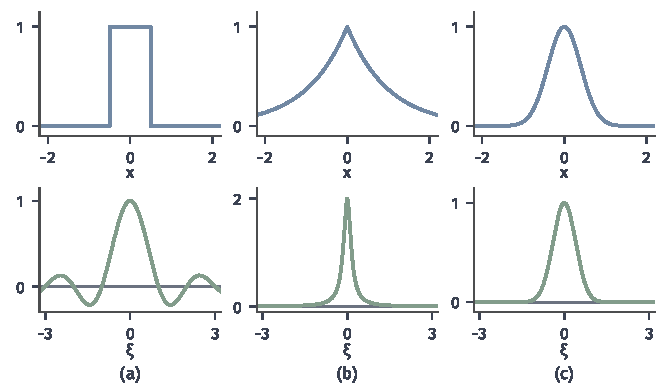
\includegraphics[width=112mm]{figures/04-spaces-measures-and-geometry/03-function-spaces/matplotlib/fourier-three-pairs/figure.pdf}
  \caption{三个Fourier变换对。上排蓝色为原函数，下排绿色为对应的变换。(a)方框$B$与$\sin(\pi\xi)/(\pi\xi)$。(b)双边指数$e^{-\lvert x\rvert}$与$2/(1+4\pi^2\xi^2)$，注意纵轴到$2$。(c)Gauss函数$e^{-\pi x^2}$与它自身。}
  \label{fig:fourier-three-pairs}
\end{BookInlineFigure}

\paragraph{平移、缩放与变换的定义域}

原函数作平移或缩放之后，仍属于$L^1(\mathbb R^d)$，它的变换仍是$\mathbb R^d$上全体频率的函数，变化的只是取值。例如加宽一倍的方框$B(x/2)=\mathbf 1_{[-1,1]}$，直接积分得到
\[
\widehat{B(\cdot/2)}(\xi)=\frac{\sin(2\pi\xi)}{\pi\xi},
\]
它仍定义在整条实轴上，只是零点从非零整数变成了$1/2$的非零整数倍，排得更密。具体的变换规则在第~\ref{sec:fourier-operations}节推导。

这与周期情形不同。改变周期$T$，系数所在的频率集合$\{k/T\}$本身随之改变，相当于换了一组下标。全空间上的Fourier变换没有周期可改，频率集合总是整个$\mathbb R^d$；函数支撑的大小不决定变换的定义域，只影响变换的形状。

\subsection{反演的条件}
\label{sec:fourier-l1-inversion}

变换对每个可积函数都存在，但从$\widehat f$还原$f$是另一个问题。在有限维中，酉矩阵的逆就是共轭转置。这提示最自然的候选：把指数的符号反过来再积分，即对函数$h$定义\term{逆Fourier变换}（inverse Fourier transform）
\begin{equation}
\check h(x)=\int_{\mathbb R^d}h(\xi)e^{2\pi\mathrm ix\cdot\xi}\,\mathrm d\xi .
\label{eq:fourier-inverse}
\end{equation}

如果直接把$\widehat f$的定义代入式~\eqref{eq:fourier-inverse}并交换积分次序，会得到内层积分$\int e^{2\pi\mathrm i(x-y)\cdot\xi}\,\mathrm d\xi$。在矩阵的类比中，这应是单位矩阵的$(x,y)$元，可是这个积分根本不收敛，因为被积函数的模恒为$1$。类比到此失效，反演不能由“$U^*U=I$”直接读出。

方框的例子表明困难是实在的：$\widehat B$不绝对可积，式~\eqref{eq:fourier-inverse}作为Lebesgue积分根本不存在。本小节先在$\widehat f$也可积的条件下建立反演，再讨论更弱条件下的逐点版本。

\paragraph{Gauss核的恒等逼近}

反演的证明不直接处理发散的内层积分，而是在频域乘一个缓慢消失的因子$G(t\xi)$，使一切积分绝对收敛，最后再令$t\to0$。为此引入缩放的Gauss核
\[
G_t(x)=t^{-d}G(x/t),\qquad t>0.
\]
作换元$x=tu$，得到$\int G_t=1$；$t$越小，$G_t$越集中在原点附近。

下面算$G(t\xi)$的逆变换。换元$\eta=t\xi$，再用$G$是偶函数且$\widehat G=G$，得到
\begin{equation}
\int_{\mathbb R^d}G(t\xi)e^{2\pi\mathrm iz\cdot\xi}\,\mathrm d\xi=t^{-d}\,\widehat G(-z/t)=G_t(z).
\label{eq:fourier-gauss-kernel-inverse}
\end{equation}
所以内层那个发散的积分，乘上$G(t\xi)$后就变成了集中在$z=0$附近的$G_t(z)$，这正是“单位矩阵的元”应有的样子。

\begin{lemma}[Gauss核的恒等逼近]
\label{lem:fourier-gauss-approx}
设$f\in L^1(\mathbb R^d)$，$t>0$，记$(f*G_t)(x)=\int f(y)G_t(x-y)\,\mathrm dy$。则
\begin{enumerate}
\item 对每个$x$，
\begin{equation}
\int_{\mathbb R^d}\widehat f(\xi)G(t\xi)e^{2\pi\mathrm ix\cdot\xi}\,\mathrm d\xi=(f*G_t)(x);
\label{eq:fourier-gauss-regularized}
\end{equation}
\item $t\to0$时$\lVert f*G_t-f\rVert_1\to0$。
\end{enumerate}
\end{lemma}

\begin{proof}
第1条。先确认可以交换积分次序：
\[
\int\!\!\int\lvert f(y)\rvert\,G(t\xi)\,\mathrm dy\,\mathrm d\xi=t^{-d}\lVert f\rVert_1<\infty.
\]
于是可以用Fubini定理，再用式~\eqref{eq:fourier-gauss-kernel-inverse}，得到
\[
\begin{aligned}
\int\widehat f(\xi)G(t\xi)e^{2\pi\mathrm ix\cdot\xi}\,\mathrm d\xi
&=\int f(y)\Bigl(\int G(t\xi)e^{2\pi\mathrm i(x-y)\cdot\xi}\,\mathrm d\xi\Bigr)\mathrm dy\\
&=\int f(y)G_t(x-y)\,\mathrm dy.
\end{aligned}
\]

第2条。由$\int G_t=1$，把$f(x)$写进积分，得到
\[
(f*G_t)(x)-f(x)=\int G_t(h)\bigl(f(x-h)-f(x)\bigr)\,\mathrm dh.
\]
取绝对值后对$x$积分，用Tonelli定理交换次序，再换元$h=tu$，记$(\tau_hf)(x)=f(x-h)$，得到
\[
\lVert f*G_t-f\rVert_1\leq\int G_t(h)\lVert\tau_hf-f\rVert_1\,\mathrm dh=\int G(u)\lVert\tau_{tu}f-f\rVert_1\,\mathrm du.
\]
被积函数被$2\lVert f\rVert_1G(u)$控制，且由平移积分连续性逐点趋于零，控制收敛定理给出结论。
\end{proof}

像$G_t$这样非负、积分为$1$、质量随参数集中到原点的核族称为\term{恒等逼近}（approximate identity）：与它卷积几乎不改变函数。第~\ref{chap:smoothing-weak-derivatives}章的磨光核也是恒等逼近，Gauss核的好处是它的Fourier变换可以精确算出。

式~\eqref{eq:fourier-gauss-regularized}的两边分别在频域和空间中描述同一件事，图~\ref{fig:fourier-gauss-smoothing}以方框为例。频域中，$\widehat B$乘上$G(t\xi)$后，高频部分被压掉，积分收敛了；空间中，这对应把方框的跳跃抹平。$t$越小，频域保留的范围越宽，空间中抹平的范围越窄，最终回到原函数。

\begin{BookInlineFigure}
  \centering
  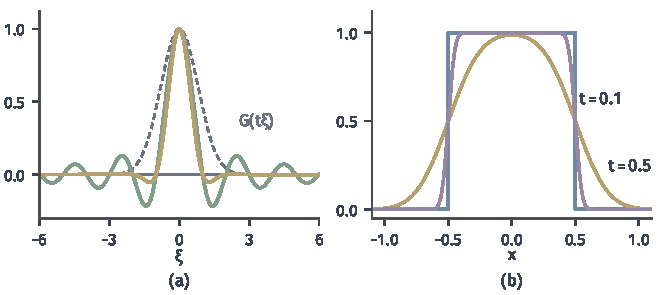
\includegraphics[width=112mm]{figures/04-spaces-measures-and-geometry/03-function-spaces/matplotlib/fourier-gauss-smoothing/figure.pdf}
  \caption{频域乘$G(t\xi)$与空间卷积$G_t$是同一运算，这里$f=B$。(a)绿色为$\widehat B$，灰色虚线为$G(t\xi)$（$t=0.5$），黄色为乘积。(b)蓝色为方框$B$，黄色与紫色为$B*G_t$，$t=0.5$与$t=0.1$；$t$越小，曲线越贴近方框。}
  \label{fig:fourier-gauss-smoothing}
\end{BookInlineFigure}

\paragraph{反演定理}

有了引理，令$t\to0$：左边在$\widehat f$可积时趋于逆变换，右边趋于$f$，反演就得到了。

\begin{theorem}[$L^1$反演定理]
\label{thm:fourier-l1-inversion}
设$f\in L^1(\mathbb R^d)$且$\widehat f\in L^1(\mathbb R^d)$。令
\begin{equation}
g(x)=\int_{\mathbb R^d}\widehat f(\xi)e^{2\pi\mathrm ix\cdot\xi}\,\mathrm d\xi ,
\label{eq:fourier-l1-inversion}
\end{equation}
则$g$是在无穷远处趋于零的连续函数，并且$f=g$几乎处处。若$f$在点$x_0$处连续，则$f(x_0)=g(x_0)$。
\end{theorem}

\begin{proof}
换元$\xi\mapsto-\xi$可知$g$是可积函数$\xi\mapsto\widehat f(-\xi)$的Fourier变换，由定理~\ref{thm:fourier-l1-properties}，它连续且在无穷远处趋于零。

在式~\eqref{eq:fourier-gauss-regularized}中令$t\to0$。左边的被积函数逐点趋于$\widehat f(\xi)e^{2\pi\mathrm ix\cdot\xi}$，并被可积函数$\lvert\widehat f\rvert$控制，所以左边对每个$x$趋于$g(x)$。

另一方面，引理~\ref{lem:fourier-gauss-approx}第2条说明$f*G_t\to f$于$L^1$。按$L^1$收敛的序列有几乎处处收敛的子列（第~\ref{chap:function-normed-spaces}章），所以沿某个子列$t_n\to0$，$(f*G_{t_n})(x)\to f(x)$对几乎每个$x$成立。两个极限相等，故$f=g$几乎处处。

若$f$在$x_0$处连续，对$\varepsilon>0$取$r>0$，使$\lvert x-x_0\rvert<r$时
\[
\lvert f(x)-f(x_0)\rvert<\varepsilon,\qquad\lvert g(x)-g(x_0)\rvert<\varepsilon.
\]
这个球的测度为正，其中有点$x$满足$f(x)=g(x)$，所以$\lvert f(x_0)-g(x_0)\rvert<2\varepsilon$。由$\varepsilon$任意，得到$f(x_0)=g(x_0)$。
\end{proof}

定理有三层含义。第一，反演公式给出的是$f$的一个连续代表，原函数作为等价类与它相等。第二，凡是$\widehat f$可积的$f$，必与一个连续函数几乎处处相等；方框有跳跃，所以$\widehat B$不可积，这与前面的直接计算一致。第三，变换是单射：若$\widehat f=\widehat g$，则$\widehat{f-g}=0$可积，反演给出$f=g$几乎处处，这相当于有限维中“坐标全同则向量相同”。

双边指数满足定理的条件，而且处处连续，所以反演对每个$x$成立：
\[
e^{-\lvert x\rvert}=\int_{\mathbb R}\frac{2}{1+4\pi^2\xi^2}\,e^{2\pi\mathrm ix\xi}\,\mathrm d\xi.
\]
在$x=0$处检验。作换元$u=2\pi\xi$，右边变成
\[
\int_{\mathbb R}\frac{2}{1+4\pi^2\xi^2}\,\mathrm d\xi=\frac1\pi\int_{\mathbb R}\frac{\mathrm du}{1+u^2}=1,
\]
与左边的$e^0=1$一致。

\paragraph{逐点反演与对称截断}

$\widehat f$不可积时，式~\eqref{eq:fourier-inverse}只能理解为某种极限。一维中最常用的是对称截断。对有限的$R$，积分区间有界，Fubini定理可用，内层积分算出来是
\[
\int_{-R}^{R}e^{2\pi\mathrm i(x-y)\xi}\,\mathrm d\xi=\frac{\sin\bigl(2\pi R(x-y)\bigr)}{\pi(x-y)}.
\]
再换元$t=x-y$，得到
\begin{equation}
\int_{-R}^{R}\widehat f(\xi)e^{2\pi\mathrm ix\xi}\,\mathrm d\xi=\int_{\mathbb R}f(x-t)\,\frac{\sin(2\pi Rt)}{\pi t}\,\mathrm dt .
\label{eq:fourier-symmetric-truncation}
\end{equation}
这里的核$\sin(2\pi Rt)/(\pi t)$扮演Dirichlet核的角色。下面需要它的积分，也就是Dirichlet积分
\[
\int_0^\infty\frac{\sin s}{s}\,\mathrm ds=\frac\pi2.
\]

Dirichlet积分可以用周期情形的工具算出。由$\frac1{2\pi}\int_0^\pi D_N=\frac12$和式~\eqref{eq:fourier-dirichlet-closed}，得到
\[
\int_0^\pi\frac{\sin\bigl((N+\tfrac12)t\bigr)}{\sin(t/2)}\,\mathrm dt=\pi.
\]
函数$\frac1{\sin(t/2)}-\frac2t$在$(0,\pi]$上有界（$t\to0$时趋于零），由Riemann--Lebesgue引理，把分母换成$t/2$不改变极限。作换元$s=(N+\tfrac12)t$，于是
\[
\lim_{N\to\infty}\int_0^{(N+1/2)\pi}\frac{\sin s}{s}\,\mathrm ds=\frac\pi2.
\]
反常积分$\int_0^\infty\frac{\sin s}{s}\,\mathrm ds$由分部积分知收敛，极限沿这个子列读出，就是$\pi/2$。

\begin{theorem}[对称截断的逐点反演]
\label{thm:fourier-symmetric-inversion}
设$f\in L^1(\mathbb R)$，并且在每个有界区间上都是分段$C^1$的。则对每个$x$，
\begin{equation}
\lim_{R\to\infty}\int_{-R}^{R}\widehat f(\xi)e^{2\pi\mathrm ix\xi}\,\mathrm d\xi=\frac{f(x+)+f(x-)}2 .
\label{eq:fourier-symmetric-inversion}
\end{equation}
\end{theorem}

\begin{proof}
核$\sin(2\pi Rt)/(\pi t)$是偶函数，所以式~\eqref{eq:fourier-symmetric-truncation}的右边可以写成$(0,\infty)$上的积分，被积函数含$f(x+t)+f(x-t)$。把积分在$t=1$处分开，并在$(0,1)$上减去左右极限，得到三项：
\[
\begin{aligned}
&\int_1^\infty\frac{f(x+t)+f(x-t)}{\pi t}\sin(2\pi Rt)\,\mathrm dt\\
&\quad+\int_0^1\frac{h(t)}{\pi t}\sin(2\pi Rt)\,\mathrm dt\\
&\quad+\bigl(f(x+)+f(x-)\bigr)\int_0^1\frac{\sin(2\pi Rt)}{\pi t}\,\mathrm dt,
\end{aligned}
\]
其中$h(t)=f(x+t)-f(x+)+f(x-t)-f(x-)$。

第一项的被积系数在$(1,\infty)$上可积，因为$f\in L^1$且$1/t\leq1$。第二项的被积系数在$(0,1)$上有界：靠近$t=0$处用定理~\ref{thm:fourier-dirichlet}证明中的单侧Lipschitz估计，其余部分用$f$在有界区间上有界。由引理~\ref{lem:fourier-riemann-lebesgue}，这两项都趋于零。

第三项作换元$s=2\pi Rt$，由Dirichlet积分，得到
\[
\int_0^1\frac{\sin(2\pi Rt)}{\pi t}\,\mathrm dt=\frac1\pi\int_0^{2\pi R}\frac{\sin s}{s}\,\mathrm ds\to\frac12.
\]
\end{proof}

对方框$B$，这一结论在$x=\pm1/2$处给出$1/2$，在其余点给出$B(x)$，这是Dirichlet定理在全空间上的对应结果。

本节的两个问题要分开看待。变换的存在只需要$f\in L^1$，在每个频率处都有确定的值。反演则另需条件：$\widehat f\in L^1$时反演积分绝对收敛，结论在几乎处处意义下成立；只有局部正则性时，要先规定积分的极限方式，结论在每一点成立，跳跃点处得到平均值。
